%%%%%%%%%%%
% METHODS %
%%%%%%%%%%%

\section{Methods}

\subsection{Neural Networks}

% MNIST CNN
%\begin{figure}[h!]
\begin{figure}[h]
    \centering
    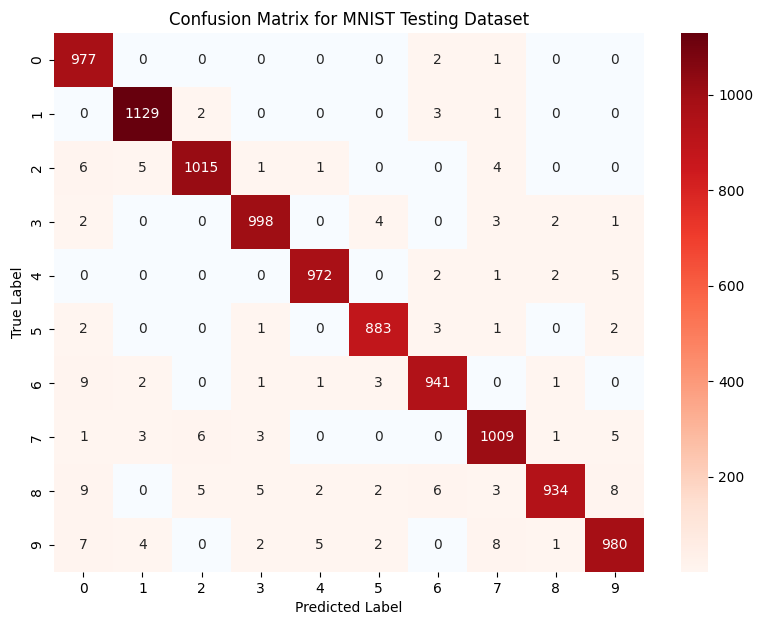
\includegraphics[width=0.99\columnwidth]{Figures/mnist_testing_dataset_confusion_matrix.png}   %\captionsetup{justification=raggedright,singlelinecheck=false}
    \caption{MNIST testing dataset confusion matrix where the least misclassified digit is 0 (top row) and the most misclassified digit is 8 (second row from bottom up), where the figures represent a snapshot i.e. one single testing dataset, the main difference between a traditional confusion matrix and the MLM which may represent n distribution-shifted testing datasets.}
\label{fig:mnist_testing_dataset_confusion_matrix}
\end{figure}

A Convolutional Neural Network (CNN) is used to classify handwritten digits from the MNIST dataset, consisting of 60,000 training images and 10,000 testing images, each of size 28x28 grayscale (single channel) pixels, representing digits from 0 to 9.

% We study not only the highest probability score (prediction), but the entire neural network output vector $\mathbf{p} = (p_1, p_2, \dots, p_K)$ where $\sum p_i = 1$, representing a probability distribution obtained by normalizing the logit vector $\mathbf{z} = (z_1, z_2, \dots, z_K)$ through the softmax function, $p_i = \text{softmax}(z_i) = e^{z_i} / \sum_{j=1}^{K} e^{z_j}$. For example, given $\mathbf{p} = [0.01, 0.01, 0.01, 0.01, 0.9, 0.01, 0.01, 0.01, 0.01, 0.01]$, the predicted class is '4', corresponding to the highest value at index five, reflecting the confidence of the prediction for each class from '0' to '9'. The logits, representing log-likelihoods of class memberships, are related to probabilities by $z_i = \log (p_i / (1 - p_i))$ where $z_i$ is the logit for class $i$, and $p_i$ is the probability of the input belonging to class $i$\cite{goodfellow2016deep, bishop2006pattern}.

In our analysis, we consider the classifier neural network's entire output, not just the highest probability score. The network produces a probability vector $\mathbf{p} = (p_1, p_2, \dots, p_K)$, where $\sum p_i = 1$,

This probability distribution is derived from a logit vector $\mathbf{z} = (z_1, z_2, \dots, z_K)$ through the application of the softmax function:

\begin{equation}
p_i = \text{softmax}(z_i) = \frac{e^{z_i}}{\sum_{j=1}^{K} e^{z_j}}
\end{equation}

For example, given 

$\mathbf{p} = [0.01, 0.01, 0.01, 0.01, 0.9, 0.01, 0.01, 0.01, 0.01, 0.01]$, the predicted class is '4', corresponding to the highest value at index five, reflecting the confidence of the prediction for each class from '0' to '9'.

The relationship between logits and probabilities can be expressed as:

\begin{equation}
z_i = \log \left(\frac{p_i}{1 - p_i}\right)
\end{equation}

Here, $z_i$ represents the logit for class $i$, while $p_i$ denotes the probability that the input belongs to class $i$. These logits can be interpreted as log-likelihoods of class membership \cite{goodfellow2016deep, bishop2006pattern}.

By examining the entire output vector, rather than just the highest score, we gain deeper insights into the model's decision-making process and its level of certainty or uncertainty across all possible classes.

The CNN architecture, implemented using PyTorch, consists of two convolutional layers followed by two fully connected layers. The first convolutional layer has 16 filters with a kernel size of 3x3 and a padding of 1. The second convolutional layer has 32 filters with the same kernel size and padding. Each convolutional layer is followed by a ReLU activation function and a max-pooling layer with a pool size of 2x2. The output of the second convolutional layer is flattened and passed through two fully connected layers with 128 and 10 neurons, respectively. The final output is passed through a log-softmax function to obtain the predicted class probabilities. The total number of parameters for the CNN MNIST classifier is 206,922.

The model was trained using the Stochastic Gradient Descent (SGD) optimizer with a learning rate of 0.01, batch size of 64 and Cross-Entropy loss function. %The learning rate was determined using a custom learning rate function that decreases the learning rate over time. The Cross-Entropy Loss function was used as the criterion for optimization. 

%%%%%%%%%%%%%%%%%%%%%%%%%%%
% PERTURBED MNIST DATASET %
%%%%%%%%%%%%%%%%%%%%%%%%%%%

\subsection{Perturbed MNIST Dataset}
\label{methods:PerturbedMNISTDataset}

% To test our trained model, we augment the MNIST testing dataset, consisting of 10,000 images with 10 classes of approximately 1,000 examples each. We create 12 perturbations - Brightness, Contrast, Defocus Blur, Fog, Frost, Gaussian Noise, Impulse Noise, Motion Blur, Pixelation, Shot Noise, Snow and Zoom Blur - following prior work by \cite{hendrycks2019benchmarking}, at 10 intensity levels, generating a dataset of 1,210,000 images. We modify perturbation function parameters by trial and error such that increased perturbation levels on the testing dataset cause network predictive accuracies to decrease linearly.

To test our trained model, we augment by two orders of magnitude the MNIST testing dataset, where the original testing dataset consists of 10,000 images with 10 classes of approximately 1,000 examples each. We create 12 perturbations - Brightness, Contrast, Defocus Blur, Fog, Frost, Gaussian Noise, Impulse Noise, Motion Blur, Pixelation, Shot Noise, Snow and Zoom Blur - following prior work by \cite{hendrycks2019benchmarking}, at 10 intensity levels, generating a dataset of 1,210,000 images. We modify perturbation function parameters by trial and error such that increased perturbation levels on the testing dataset cause network predictive accuracies to decrease linearly. The 60,000 image training dataset was left unperturbed. While it would be desirable to use more than one dataset, it has been demonstrated that softmax output distances to centroids (explained in the next section) are greater for misclassified examples in both MNIST/CNN and CIFAR-10/ViT (Vision Transformer) \cite{sikar2024acceptautomatedpredictionsdefer}. CNNs have been the traditional go-to architecture for image recognition tasks, leveraging local receptive fields and spatial hierarchies. Vision Transformers, on the other hand, represent a more recent paradigm shift in computer vision, adapting the self-attention mechanism from natural language processing to image analysis. Despite these fundamental differences in architecture, both types of models exhibit similar behavior in terms of the relationship between softmax output distances and misclassification likelihood. 

It is also important to note that the probability distribution of a digit belonging to a class is not normally distributed, but rather follows a multinomial distribution across the 10 digit classes.
% the line above in reply to referee 2:
% Technical Soundness: The key technical element is to specify misclassification as the (normalised) reciprocal of distance, d,  of some datum x to some class c. In most cases the distance d would be used as a probability measure of the class generating the datum, eg p( x | c ) = N(  d | c ), with N the Normal distribution.  The posterior would then be formed p( c | x  ) as the probability that x belongs to c

%%%%%%%%%%%%%%%%%%%%%%%%%%%%%%%%%%%%%%%
% MISCLASSIFICATION LIKELIHOOD MATRIX %
%%%%%%%%%%%%%%%%%%%%%%%%%%%%%%%%%%%%%%%

\subsection{Misclassification Likelihood Matrix}
\label{miss_class_matrix}

\begin{figure}[h]
    \centering
    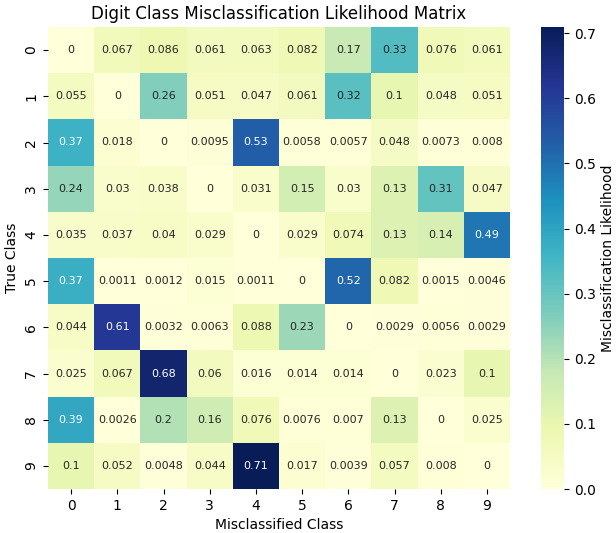
\includegraphics[width=0.99\columnwidth]{Figures/DigitClassMisclassificationLikelihoodMatrix.png}   %\captionsetup{justification=raggedright,singlelinecheck=false}
    \caption{Perturbed MNIST testing dataset MLM, where dark blue indicates greater, and lighter yellow lower likelihood of misclassification. The figures effectively represent 120 MNIST testing datasets with 10 levels of noise across 12 different perturbation types.} 
    \label{fig:DigitClassMisclassificationLikelihoodMatrix}
\end{figure}

To generate a Misclassification Likelihood Matrix for a particular model and dataset, we proceed as described next:

\textbf{a}. Obtaining the Centroids:
Let $ D = {(x_1, y_1), (x_2, y_2), ..., (x_n, y_n)} $ be the training dataset, where $ x_i \in \mathbb{R}^d $ represents the input features and $y_i \in {0, 1, ..., 9}$ represents the corresponding digit class label. We train a neural network classifier $f_\theta(x)$ on this dataset, where $\theta$ represents the learned parameters of the model.
To obtain the initial class centroids, we first collect the softmax outputs of the trained classifier for each correctly classified example in the training set. Let $S_c = {s_1, s_2, ..., s_m}$ be the set of softmax outputs for examples correctly classified as class $c$, where $s_i \in \mathbb{R}^{10}$. We calculate the initial centroid $\mu_c$ for class $c$ as the mean of the softmax outputs:

\begin{equation}
\mu_c = \frac{1}{m} \sum_{i=1}^m s_i
\label{eq:mean_softmax_output}
\end{equation}

We repeat this process for each digit class $c \in {0, 1, ..., 9}$ to obtain the initial centroids $\mu_0, \mu_1, ..., \mu_9$.

After obtaining the initial centroids, we use them to initialize the K-Means algorithm. The K-Means algorithm iteratively assigns each softmax output to the nearest centroid and updates the centroids based on the assigned outputs until convergence. This process refines the centroids and yields the final adjusted centroids $\hat{\mu}_0, \hat{\mu}_1, ..., \hat{\mu}_9$.

\textbf{b}. Obtaining the Distance to a Neighboring Centroid:
Given a test example $x$ with true class label $y$, we obtain the softmax output $s = f_\theta(x)$, that we interpret as points in a simplex, which has a natural Euclidean geometry. To calculate the distance between $s$ and a neighboring class centroid $\hat{\mu}c$, where $c \neq y$, we use the Euclidean distance:
% statement about euclidean distance in reply to referee 1:
%  Or why softmax outputs are already in Euclidean metric space?

\begin{equation}
d(s, \hat{\mu}c) = \sqrt{\sum\limits_{i=1}^{10} (s_i - \hat{\mu}{c,i})^2}
\label{eq:euclidean_distance_to_neighboring_centroid}
\end{equation}

This distance measures how close the softmax output of the test example is to the adjusted centroid of a different class.

\textbf{c}. Obtaining the Nearest Distances Between Digit Classes Matrix:
To construct the matrix of nearest distances between digit classes, we iterate over all test examples and calculate the nearest distance to each neighboring class centroid. Let $X_y$ be the set of test examples with true class label $y$. For each test example $x \in X_y$, we calculate the distance $d(f_\theta(x), \hat{\mu}c)$ to each neighboring class centroid $\hat{\mu}c$, where $c \neq y$.
We then find the minimum distance among all test examples in $X_y$ to each neighboring class centroid:
\begin{equation}
D{y,c} = \min{x \in X_y} d(f_\theta(x), \hat{\mu}c)
\label{eq:min_distance_to_near_centroid}
\end{equation}
The resulting matrix $D \in \mathbb{R}^{10 \times 10}$ contains the nearest distances between each pair of digit classes, where $D{y,c}$ represents the nearest distance from class $y$ to class $c$.

\textbf{d}. Obtaining the Misclassification Likelihood Matrix:
To obtain the misclassification likelihood matrix, we transform the nearest distance matrix $D$ by taking the reciprocal of each element and normalizing the rows:
\begin{equation}
L_{y,c} = \frac{\frac{1}{D_{y,c}}}{\sum\limits_{c=0}^9 \frac{1}{D_{y,c}}}
\label{eq:reciprocal_distance_matrix_eg_likelihood_matrix}
\end{equation}

The resulting matrix $L \in \mathbb{R}^{10 \times 10}$ contains the misclassification likelihoods between each pair of digit classes, where $L_{y,c}$ represents the likelihood of an example from class $y$ being misclassified as class $c$. Higher values indicate a higher likelihood of misclassification, while lower values indicate a lower likelihood.

% \subsection{rewrite own lines}

% Sure, here is the revised version with important equations on their own lines:

% ---

% ### a. Obtaining the Centroids:

% Let \( D = \{(x_1, y_1), (x_2, y_2), \ldots, (x_n, y_n)\} \) be the training dataset, where \( x_i \in \mathbb{R}^d \) represents the input features and \( y_i \in \{0, 1, \ldots, 9\} \) represents the corresponding digit class label. We train a neural network classifier \( f_\theta(x) \) on this dataset, where \(\theta\) represents the learned parameters of the model.

% To obtain the initial class centroids, we first collect the softmax outputs of the trained classifier for each correctly classified example in the training set. Let \( S_c = \{s_1, s_2, \ldots, s_m\} \) be the set of softmax outputs for examples correctly classified as class \(c\), where \( s_i \in \mathbb{R}^{10} \). We calculate the initial centroid \( \mu_c \) for class \(c\) as the mean of the softmax outputs:

% \[
% \mu_c = \frac{1}{m} \sum_{i=1}^m s_i
% \]

% We repeat this process for each digit class \( c \in \{0, 1, \ldots, 9\} \) to obtain the initial centroids \( \mu_0, \mu_1, \ldots, \mu_9 \).

% After obtaining the initial centroids, we use them to initialize the KMeans algorithm. The KMeans algorithm iteratively assigns each softmax output to the nearest centroid and updates the centroids based on the assigned outputs until convergence. This process refines the centroids and yields the final adjusted centroids \( \hat{\mu}_0, \hat{\mu}_1, \ldots, \hat{\mu}_9 \).

% ### b. Obtaining the Distance to a Neighboring Centroid:

% Given a test example \(x\) with true class label \(y\), we obtain the softmax output \(s = f_\theta(x)\). To calculate the distance between \(s\) and a neighboring class centroid \( \hat{\mu}_c \), where \( c \neq y \), we use the Euclidean distance:

% \[
% d(s, \hat{\mu}_c) = \sqrt{\sum_{i=1}^{10} (s_i - \hat{\mu}_{c,i})^2}
% \]

% This distance measures how close the softmax output of the test example is to the adjusted centroid of a different class.

% ### c. Obtaining the Nearest Distances Between Digit Classes Matrix:

% To construct the matrix of nearest distances between digit classes, we iterate over all test examples and calculate the nearest distance to each neighboring class centroid. Let \( X_y \) be the set of test examples with true class label \(y\). For each test example \( x \in X_y \), we calculate the distance \( d(f_\theta(x), \hat{\mu}_c) \) to each neighboring class centroid \( \hat{\mu}_c \), where \( c \neq y \).

% We then find the minimum distance among all test examples in \( X_y \) to each neighboring class centroid:

% \[
% D_{y,c} = \min_{x \in X_y} d(f_\theta(x), \hat{\mu}_c)
% \]

% The resulting matrix \( D \in \mathbb{R}^{10 \times 10} \) contains the nearest distances between each pair of digit classes, where \( D_{y,c} \) represents the nearest distance from class \(y\) to class \(c\).

% ### d. Obtaining the Misclassification Likelihood Matrix:

% To obtain the misclassification likelihood matrix, we transform the nearest distance matrix \(D\) by taking the reciprocal of each element and normalizing the rows:

% \[
% L_{y,c} = \frac{\frac{1}{D_{y,c}}}{\sum_{c=0}^9 \frac{1}{D_{y,c}}}
% \]

% The resulting matrix \( L \in \mathbb{R}^{10 \times 10} \) contains the misclassification likelihoods between each pair of digit classes, where \( L_{y,c} \) represents the likelihood of an example from class \(y\) being misclassified as class \(c\). Higher values indicate a higher likelihood of misclassification, while lower values indicate a lower likelihood.

% ---

% This formatting places each key equation on its own line for clarity.

\subsection{Testing the hypothesis}

To test the hypothesis that some misclassifications are more likely to occur than others, we can analyze how the misclassification likelihoods change as we introduce perturbations to the input images. By comparing the misclassification likelihoods at different perturbation levels, we can determine if certain digit pairs are consistently more prone to misclassification.

Let $L^{(p)} \in \mathbb{R}^{10 \times 10}$ be the misclassification likelihood matrix at perturbation level $p$, where $p \in \{1, 2, ..., 10\}$. Each element $L^{(p)}_{y,c}$ represents the likelihood of an example from class $y$ being misclassified as class $c$ at perturbation level $p$.

To obtain $L^{(p)}$, we follow a similar process as described in Section \ref{miss_class_matrix}.d, but we use the distances calculated from the perturbed examples at level $p$. Let $X^{(p)}_y$ be the set of test examples with true class label $y$ at perturbation level $p$. For each test example $x \in X^{(p)}_y$, we calculate the distance $d(f_\theta(x), \mu_c)$ to each neighboring class centroid $\mu_c$, where $c \neq y$.

We then find the minimum distance among all test examples in $X^{(p)}_y$ to each neighboring class centroid:

\begin{equation}
D^{(p)}_{y,c} = \min_{x \in X^{(p)}_y} d(f_\theta(x), \mu_c)    
\end{equation}

The resulting matrix $D^{(p)} \in \mathbb{R}^{10 \times 10}$ contains the nearest distances between each pair of digit classes at perturbation level $p$.

To obtain the misclassification likelihood matrix $L^{(p)}$, we apply the same transformation as in Section \ref{miss_class_matrix}.d:
\begin{equation}
L^{(p)}_{y,c} = \frac{\frac{1}{D^{(p)}_{y,c}}}{\sum\limits_{c=0}^9 \frac{1}{D^{(p)}_{y,c}}}    
\end{equation}

We repeat this process for each perturbation level $p$ to obtain a set of misclassification likelihood matrices $\{L^{(1)}, L^{(2)}, ..., L^{(10)}\}$.

To test the hypothesis, we can analyze the changes in misclassification likelihoods across different perturbation levels. We can calculate the average misclassification likelihood for each digit pair $(y, c)$ across all perturbation levels:
\begin{equation}
\bar{L}_{y,c} = \frac{1}{10} \sum_{p=1}^{10} L^{(p)}_{y,c}    
\end{equation}

We can then identify the digit pairs with the highest average misclassification likelihoods. If these pairs consistently have high misclassification likelihoods across different perturbation levels, it suggests that they are more prone to misclassification compared to other digit pairs.

To quantify the consistency of misclassification likelihoods across perturbation levels, we can calculate the standard deviation of the misclassification likelihoods for each digit pair:
\begin{equation}
\sigma_{y,c} = \sqrt{\frac{1}{10} \sum_{p=1}^{10} (L^{(p)}_{y,c} - \bar{L}_{y,c})^2}    
\end{equation}


A low standard deviation indicates that the misclassification likelihood for a digit pair remains relatively stable across perturbation levels, supporting the hypothesis that certain misclassifications are more likely to occur consistently.
